\documentclass{book}
\usepackage{graphicx}
\usepackage{amsmath}

\graphicspath{ {images/} }
\title{Maths Problems}

\author{Nicholas James}
\begin{document}
\setlength{\parskip}{6pt}
\maketitle{}
\chapter{Introductory Problems}
\section{A Singular Square}
\subsection{Problem}
\[\overline{AABB}=m^2\]

Find the four digit perfect square where both the first two digits are the same and the last two digits are the same.

\subsection{Solution}

This can be solved in a long winded way by checking whether each of the possible numbers of the form \(\overline{AABB}\) are square. However, I think we would prefer to be a little more clever about it.
Firstly, a good start with problems of this type is to write our number algebraically:

\begin{align*}
  n&=1000A+100A+10B+1B\\
  n&=1100A+11B\\
  n&=11(100A+B)
\end{align*}

So we can see that our number, \(n\), must be divisible by \(11\). Also, as \(n\) is a perfect square, we can also conclude that it must be divisible by \(11^2=121\). Let:

\begin{equation*}
n=m^2
\end{equation*}

As we know that \(n\) is divisible by \(121\) we can see that \(m\) must be divisible by \(11\). At this point we can try all the multiples of \(11\) from \(33\) to \(99\), and we will discover our answer. This has reduced our search size by more than a factor of \(10\). Continuing mathematically, we know,

\begin{equation*}
n=11(100A+B)
\end{equation*}

As \(n\) is divisible by \(121\), we can see that \(100A+B\) is divisible by \(11\). However,

\begin{equation*}
100A+B=99A+(A+B)
\end{equation*}

So, \(A+B\) must be divisible by \(11\). As \(A\) and \(B\) are both less than \(10\), \(A+B=11\). From here we have,

\begin{align*}
  n&=11(99A+11)\\
  \frac{n}{121}&=9A+1
\end{align*}

We know \(n\) is a perfect square, so \(9A+1\) must also be a perfect square. The only possibility is \(A=7 \Rightarrow 9A+1=64\). This gives us,

\begin{equation*}
n=121\times 64=7744=88^2
\end{equation*}

\newpage

\section{Selective Shaking}
\subsection{Problem}

\begin{center}

\includegraphics{handshake}
\end{center}

At a recent party, everyone shook hands exactly once with everyone else. Halfway through the party Magda arrived and shook hands only with the people she likes.

In all there were 201 handshakes.

How many people does Magda like?
\subsection{Solution}
\setlength{\parskip}{6pt}
If everyone in a group of \(n\) people shakes hands with everyone else, there are \( {{n}\choose{2}}= \frac{n(n-1)}{2}\) handshakes.
\renewcommand{\arraystretch}{1.5}
\begin{center}
\begin{tabular}{ |c|c| }

 \hline
 People at party & Handshakes \\
 \hline
 \(19\) & \({{19}\choose{2}}=171\) \\
 \(20\) & \({{20}\choose{2}}=190\) \\
 \(21\) & \({{21}\choose{2}}=210\) \\
 \hline
\end{tabular}
\end{center}

We can see that \(19\) is too few, as Magda would have to shake hands with more people than are present at the party. Similarly, \(21\) is too many, as there would have already been \(210\) handshakes before she arrived.

Therefore, there are \(20\) people at the party, and Magda likes \(201-190=\boxed{11}\) of them.
\subsection{Extension}
Is it always possible, given a total number of handshakes, to know how many people the latecomer likes?
\newpage

\section{Water into Wine}
\subsection{Problem}
\begin{center}
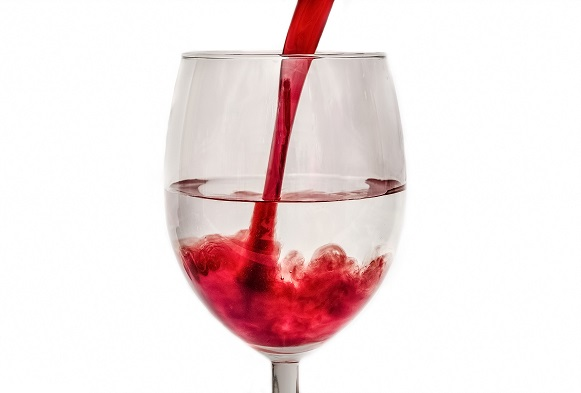
\includegraphics{wine}
\end{center}

One glass contains 100ml of water, and a second glass contains 100ml of wine. 10ml of water is taken from the first glass and put in the second. This mixture is stirred thoroughly, and 10ml is taken and placed back in the first glass.

At the end of this procedure, will the amount of wine in the first glass be greater or smaller than the amount of water in the second glass?

\subsection{Solution}
It is possible to show through a calculation that the amount of water in the second glass is the same as the amount of wine in the first glass. However, there is another way to look at this situation:

At the end of the procedure, the glasses both contain 100ml of liquid. Therefore, any water that is in the second glass must have come from the first glass, and must have been replaced in the first glass by an equal amount of wine.

\subsection{Extension}
Is it necessary to mix the contents of the second glass thoroughly?
\newpage
\section{Trigonometric Intersections}

\subsection{Problem}

What is the angle between the graphs of \(\tan x\) and \(\cos x\) at their points of intersection?
\subsection{Solution}
\subsubsection{Solution 1}
First, find the points of intersection:

\begin{align*}
\cos(x)&=\tan(x)\\
\cos(x)&=\frac{\sin(x)}{\cos(x)}\\
\cos^2(x)&=\sin(x)\\
1-\sin^2(x)&=\sin(x)
\end{align*}

Solve the quadratic to find:

\begin{equation*}
\sin(x)=\frac{1-\sqrt{5}}{2}
\end{equation*}

Happily, we don't need to find the co-ordinates. Differentiating:

\begin{align*}
d/dx(\cos(x))&=-\sin(x)\\
d/dx(\tan(x))&=-\sec^2(x)
\end{align*}

So, at the intersection, the gradient of \(\cos(x)\) is:

\begin{equation*}
-\sin(x)=-\frac{1-\sqrt{5}}{2}
\end{equation*}

Using the standard labels for a right-angled triangle (O,A,H), we know:
\begin{equation*}
\sin(x)=\frac{1-\sqrt{5}}{2}=\frac{O}{H}
\end{equation*}
\begin{equation}
H(\frac{1-\sqrt{5}}{2})=O
\end{equation}

We know from the problem:
\begin{align*}
  \frac{A}{H}&=\frac{O}{A}\\
  A^2&=OH
\end{align*}

Substitute equation (1):

\begin{align*}
  H^2(\frac{1-\sqrt{5}}{2})&=A^2\\
  \frac{H^2}{A^2}=\sec^2(x)&=\frac{2}{1-\sqrt{5}}
\end{align*}

So, we see that \(\tan(x)\) and \(\cos(x)\) are perpendicular at the intersection points, giving us an answer of \(\pi/2\) for the angle between them.
\subsubsection{Solution 2}
If we know that the tangents are perpendicular, we can prove it in a very succinct way:
\begin{align*}
  f(x)&=\cos(x)\\
  g(x)&=\tan(x)\\
  f'(x)&=-\sin(x)\\
  g'(x)&=\sec^2(x)
\end{align*}

At the points of intersection, \(f(x)=g(x)\)
\begin{align*}
  \cos(x)&=\frac{\sin(x)}{\cos(x)}\\
  1&=\frac{\sin(x)}{\cos^2(x)}
\end{align*}

So we have

\begin{equation*}
  f'(x)g'(x)=-1
\end{equation*}

Which implies the tangents at this point are perpendicular.

\section{Factorial Factors}
\subsection{Problem}
How many numbers are factors of \(21!\) but not of \(20!\)?
\subsection{Solution}
\subsubsection{Solution 1}
A naive approach would suggest that we find the prime decomposition of \(20!\)
\begin{equation*}
  20!=2^{18} \times 3^8 \times 5^4 \times 7^2 \times 11 \times 13 \times 17 \times 19
\end{equation*}
We can see the prime decomposition of \(21!\) will be the same, but with an additional \(3\) and an additional \(7\). We are therefore looking for numbers which have either \(3^9\), \(7^3\) or both as a factor. Our aim is to count the number of factors of \(21!\) that meet these criteria.

For any number we can count its factors by considering its prime composition. Take, for example:

\begin{equation*}
  n=2^x \times 3^y \times 5^z
\end{equation*}

n has \((x+1)(y+1)(z+1)\) factors. This is because there are \(x+1\) posibilities for the number of 2s in each factor (as there can be any number from 0 to x of them), and a similar thing is true for 3s and 5s.

Therefore, if we limit the factors of 21! to those which have either \(3^9\), \(7^3\) or both as a factor, we find:
\begin{center}
\begin{tabular}{ |c|c|c|c|c|c|c|c|c|c| }
\hline
Fixed & 2 & 3 & 5 & 7 & 11 & 13 & 17 & 19 & Total \\
\hline
\(3^9\) & 19 & 1 & 5 & 3 & 2 & 2 & 2 & 2 & 4560\\
\(7^3\) & 19 & 9 & 5 & 1 & 2 & 2 & 2 & 2 & 13680\\
\(3^9 \times 7^3\) & 19 & 1 & 5 & 1 & 2 & 2 & 2 & 2 & 1520\\
\hline
\end{tabular}
\end{center}
Totalling these gives us 19760 numbers which are factors of 21! but not 20!

\subsubsection{Solution 2}
We could also count the number of factors of 21! and subtract the number of factors of 20!. Using the method from solution 1 we find:
\begin{center}
\begin{tabular}{ |c|c|c|c|c|c|c|c|c|c| }
\hline
 & 2 & 3 & 5 & 7 & 11 & 13 & 17 & 19 & Total \\
\hline
\(21!\) & 19 & 10 & 5 & 4 & 2 & 2 & 2 & 2 & 60800\\
\(20!\) & 19 & 9 & 5 & 3 & 2 & 2 & 2 & 2 & 41040\\
\hline
\end{tabular}
\end{center}
Which gives us the same answer of 19760.
\subsection{Extension}
Can we use the factor finding method above to prove that only square numbers have an odd number of factors?
\newpage
\section{More or Less}
\subsection{Problem}
Do the majority of positive integers below \(10 000 000\) contain the digit \(1\)?
\subsection{Solution}
As is often the case, it's easier to count the integers below \(10000000\) which do \textbf{not} contain the digit \(1\).

This leaves \(9\) possibilities for each digit: \(0\) and \(2\) to \(9\).

So, for the integers up to 9999999, we have \(9^7-1=4782968\) integers which do not contain the digit \(1\). We had to subtract 1 because we had counted 0 among our possibilities.

Therefore, \(9999999-4782968=5217031\) integers contain the digit \(1\), which is the majority.
\subsection{Extension}
What is the first integer below which the majority of positive integers contain the digit \(1\)? (*)
\newpage
\section{Watchers on a disc}
\subsection{Problem}

\begin{center}
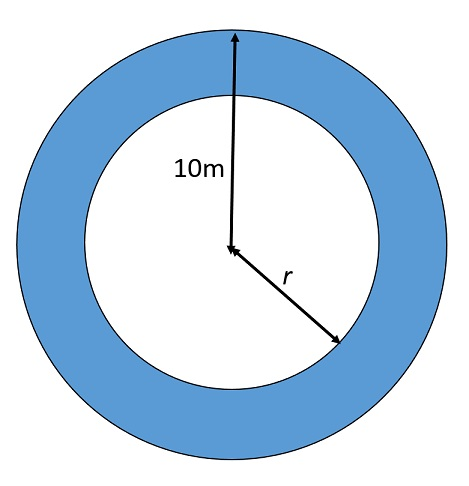
\includegraphics{annulus.jpg}
\end{center}

An art museum wants to build a new gallery. They want the floor plan to be an annulus (a ring shape bounded by two concentric circles), with the outer circle having a radius of 10m.

If they can afford to provide only \(4\) guards, who between them have to be able to see the entire gallery, what is the maximum radius of the inner circle in metres?

\subsection{Solution}
The most efficient placement of the guards would be equally spaced around the outer circle, one every \(90^{\circ}\). We want the guards to have as little overlap as possible, as we are looking for the maximum radius for the inner circle. This is achieved by having the inner circle tangent to the sides of the square formed by connecting our 4 guards.


\begin{center}
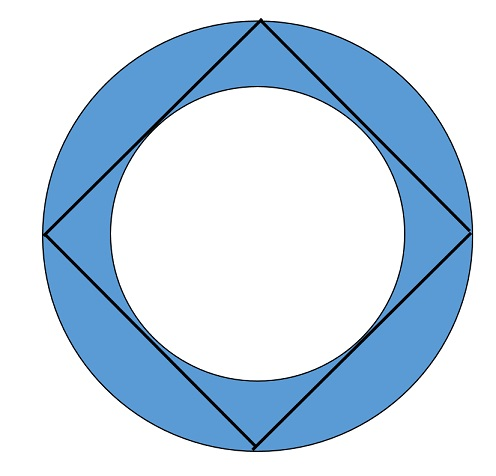
\includegraphics{annulus2}
\end{center}
If the inner circle were any larger, even in their optimal positions each of the guards would be able to see less than \(\frac{1}{4}\) of it, so at least part of the room would not be in view.

The radius of the inner circle is therefore half of the side of this square, \(s\)
\begin{align*}
  s^2+s^2&=20^2\\
  s^2&=200\\
  s&=10\sqrt{2}
\end{align*}

So, our inner radius is:

\[\frac{10\sqrt{2}}{2}=\boxed{5\sqrt{2}}\]
\subsection{Extensions}
What is the minimum number of guards?

What is the maximum inner radius if there are only 3 guards?

Can you find a formula for the maximum inner radius with n guards?
\newpage


\section{Long Multiplication}
\subsection{Problem}
\[ \begin{array} { l l l l }
& & A & B \\ \times & & & C \\ \hline & & C & B \\ \end{array} \]

If \( A, B, C \) are distinct digits that satisfy the above cryptogram, what is the value of \(B\)?
\subsection{Solution}
As \(\overline{AB}\times C = \overline{CB}\) we know that \(\overline{AB}\) must be greater than \(10\) (because it has 2 digits), but less than \(20\) (or the tens digit of the answer could not be the same as \(C\)). This means that \(A=1\).

We therefore have:

\((10+B)C=10C+B\)

\(10C+CB=10C+B\)

\((C-1)B=0\)

So, \(C=1\) or \(B=0\). As \(A=1\), \(C\neq 1\).

So \(\boxed{B=0}\)
\subsection{Extensions}
What are the possibilities for the values of \(A\) and \(C\)?

If \(A\), \(B\) and \(C\) are not necessarily distinct, what other possibilities are there for the values of \(A\), \(B\) and \(C\)?
\newpage

\section{Three Integers}
\subsection{Problem}
There exist three distinct integers \(a\), \(b\) and \(c\) such that:

\(a\), \(b\) and \(c\) is an arithmetic progression

at least one of the six permutations of \(a\), \(b\) and \(c\) is in geometric progression

\(a+b+c=3\).

What is the value of \(abc\)?
\subsection{Solution}

As \(a,b,c\) is an arithmetic progression we have:
\begin{align*}
  a&=b-r\\
  c&=b+r
\end{align*}

It's useful to define the midpoint of a series as the variable because, as in this case, it often results in the possibility of cancelling.
\begin{align*}
  a+b+c&=3\\
  (b-r)+b+(b+r)&=3\\
  3b&=3\\
  b&=1
\end{align*}

We therefore have 3 numbers: \(1-r\), \(1\) and \(1+r\). The only way these can be in geometric progression is if one is negative, and the ratio of the geometric progression is also negative. The obvious way for this to happen is if the progression is: \(1\), \(1-r\), \(1+r\).
Let \(m\) be the ratio:
\begin{align*}
  m&=1-r\\
  m^2&=1+r
\end{align*}

Squaring the first equation gives us:

\[m^2=1-2r+r^2\]

Equating:
\begin{align*}
  1-2r+r^2&=1+r\\
  r(3-r)&=0
\end{align*}

So \(r=3\) , \(a=-2,b=1,c=4\), and \(\boxed{abc=-8}\)

\newpage

\section{Triangular Breakage}

\subsection{Problem}
A uniform, straight stick is cut in two random places to make three pieces. What is the probability that these three pieces can form a triangle?

\subsection{Solution}
The key idea here is that if one of the three pieces is longer than \(\frac{1}{2}\) of the length of the stick, a triangle cannot be formed.

As the stick is uniform and straight, it is symmetrical about its midpoint. Let us define \(1\) as the length of the stick, and \(x\) as the distance of the first cut from the midpoint.
\begin{center}
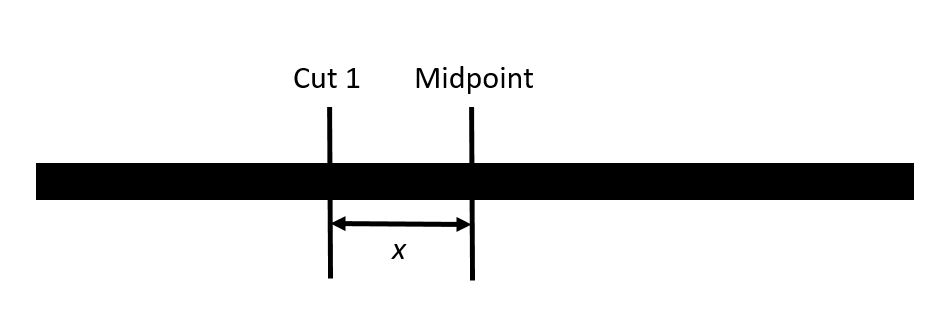
\includegraphics{stick2}
\end{center}
There are two cases:

1) The second cut is in the same half as the first. In this case there is one piece which is longer than half of the original stick. The remaining two pieces together are shorter than this, so a triangle cannot be formed.

2) The second cut is in the other half of the stick. In this case a triangle might be formed, but only if the second cut is within \(\frac{1}{2}\) of the first cut.

\begin{center}
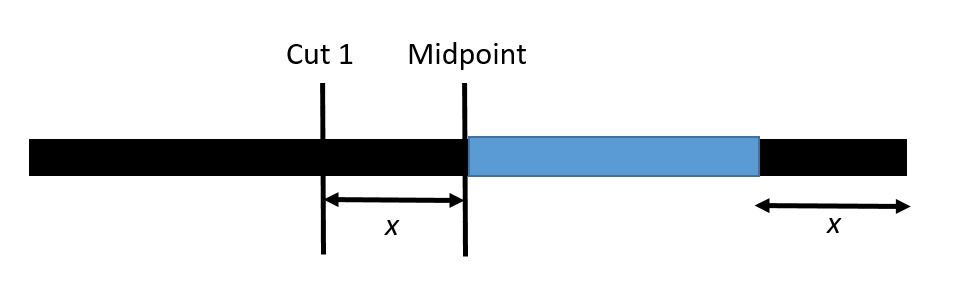
\includegraphics{stick3}
\end{center}
If the second cut is in the blue area, a triangle can be formed.

Therefore, the probability that a triangle can be formed, given a first cut at a distance \(x\) from the midpoint is:

\[P(x)= \frac{\frac{1}{2}-|x|}{1}=\frac{1}{2}-|x|\]

Graphing this, from \(x=-\frac{1}{2}\) to \(x=\frac{1}{2}\), we get:

\begin{center}
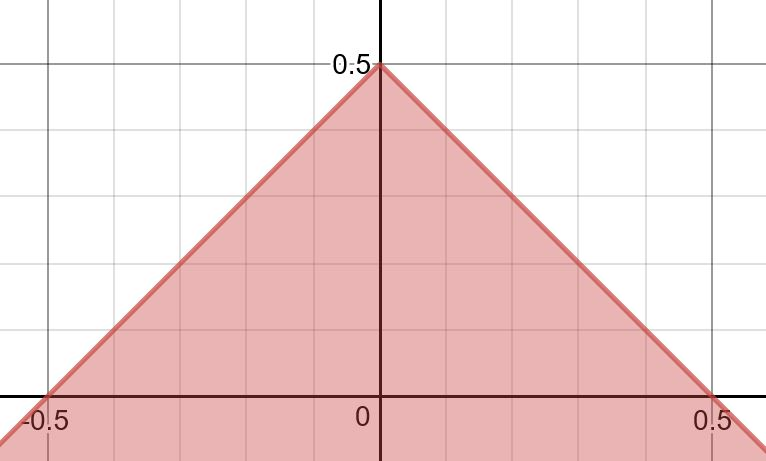
\includegraphics{stick4}
\end{center}


The area under this graph gives us our probability, so our final probability is:

\[\frac{1}{2} \times \frac{1}{2} \times 1=\boxed{\frac{1}{4}}\]
\newpage

\section{A Discerning Function}
\subsection{Problem}
Using only the operations \(+, -, \times, \div\), as well as the absolute value, or modulus, operator (\(|\:|\)), can you invent a function \(f(x,y)\) which outputs whichever is highest, \(x\) or \(y\).

\subsection{Solution}
One answer is the function:

\[f(x,y)=\frac{x+y}{2}+\frac{|x-y|}{2}\]

But how does it work?

\(\frac{x+y}{2}\) is the average of the numbers \(x\) and \(y\). Geometrically, this is the point that is halfway between \(x\) and \(y\);

\begin{center}
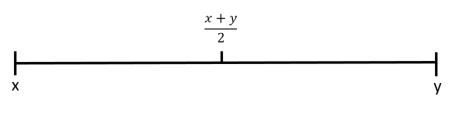
\includegraphics{function1}
\end{center}

\(|x-y|\) is the difference beteeen \(x\) and \(y\). \(\frac{|x-y|}{2}\) is half of this distance. Geometrically, if we add this to the average of \(x\) and \(y\), we will end up whichever is the highest: \(x\) or \(y\).

\begin{center}
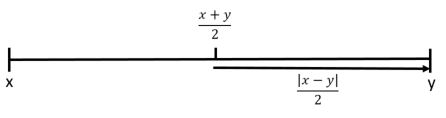
\includegraphics{function2}
\end{center}

\subsection{Extension}
How could you alter the function to output the lower of the two inputs?
\newpage

\section{Car Catastrophe}
\subsection{Problem}
Two identical cars are traveling on a road. The first car is travelling at \(25ms^{-1}\) (around 55 mph). The second car is overtaking the first at \(30ms^{-1}\) (around 65 mph).

When they are level, they both notice that the road is blocked ahead by a crashed truck. They apply their brakes at the same time.

If the first car stops just before the crashed truck, how fast (in \(ms^{-1}\)) is the second car traveling when it hits the truck?

\textbf{Assumptions}

Both cars have brakes which slow the cars at the same rate (apply an identical force).
\subsection{Solution}
It is possible to solve this question by using the uniform motion equations, and inventing either a figure for the distance to the truck, or inventing a figure for the accelleration.

A better way is to use energy. The formula for kinetic energy is \(KE=\frac{1}{2}mv^2\). At the start, the first car has kinetic energy \(E_1\):

\[E_1=\frac{1}{2}m(25)^2\]

Just before the truck, it has lost all its kinetic energy thanks to the work done by its brakes.

At the start, the second car has energy \(E_2\):

\[E_1=\frac{1}{2}m(30)^2\]

By the time it reaches the truck, it will have lost the same amount of energy as the first car, as they have both been acted on by the same force over the same distance. It will have \(E_{final}\) kinetic energy remaining:

\begin{align*}
  E_{final}&=\frac{1}{2}m(30)^2-\frac{1}{2}m(25)^2\\
  E_{final}&=\frac{1}{2}m(275)
\end{align*}


We want to find the final velocity, \(v\), so:

\begin{align*}
  \frac{1}{2}mv^2&=\frac{1}{2}m(275)\\
  v^2&=275\\
  v&=\boxed{16.58...}
\end{align*}


This is nearly \(40mph\), so the initial difference in velocities has been vastly magnified. This is because kinetic energy is proportional to \(v^2\), not simply \(v\).

\subsection{Extension}
Use the techniques you applied to this question to find out how travelling at 40mph instead of 30mph affects the stopping distance.
\newpage

\section{An Inconclusive Survey}
\subsection{Problem}
In a survey of 2000 people, 68\% of the respondents were male and the remaining 32\% were female.

If 65\% of the respondents had maths degrees, what is the minimum number of males with maths degrees?
\subsection{Solution}
Firstly note that as we do not know how the mathematics graduates are distributed among the males and females, we cannot just multiply the percentages together.

In total we know that there are \(2000 \times 0.65=1300\) mathematics graduates.

These \(1300\) mathematics graduates are either male or female. This means the minimum number of male mathematics graduates will happen when there is the maximum number of female mathematics graduates.

The maximum number of female mathematics graduates would happen if all of the female respondents were mathematics graduates. The number of female respondents is: \(2000 \times 0.32 = 640\).

So, the minimum number of male mathematics graduates is therefore \(1300-640=\boxed{660}\).
\subsection{Extensions}
What is the maximum number of male maths graduates?

What is the minimum number of female mathematics graduates?

Which more likely: that a randomly selected male is a mathematics graduate, or that a randomly selected female is a mathematics graduate?
\newpage

\section{Prime Factors?}
\subsection{Problem}
Each prime number, \(p\), has precisely two factors, 1 and \(p\). How many non-prime positive integers under 1000 have a prime number of factors?

For example, 4 is a non-prime positive integer under 1000 with 3 (which is a prime number) factors 1, 2, and 4.

\subsection{Solution}
All integers can be written uniquely as the product of their prime factors:

\[n=A^a \times B^b \times C^c \times ...\]

Where \(A,B,C,...\) are prime numbers, and \(a,b,c...\geq 1\).

This number, \(n\), has \((a+1)(b+1)(c+1)...\) factors in total.

As \(a,b,c...\geq 1\), \((a+1),(b+1),(c+1)...\geq 2\).

We can see from this that if a number has more than one prime factor it must have a composite number of factors, as its total number of factors will be the product of two or more numbers.

We are therefore looking for numbers with only one prime factor, i.e. \(n=p^y\), where \(p\) is a prime, and \(y \geq 2\), as the question excludes prime numbers.

These numbers, \(n=p^y\), have \(y+1\) factors.
\newpage
We are therefore looking for primes raised to powers which are one less than a prime number, eg. \(2,4,6,10..\).  The result of this must also be less than \(1000\):

\begin{center}
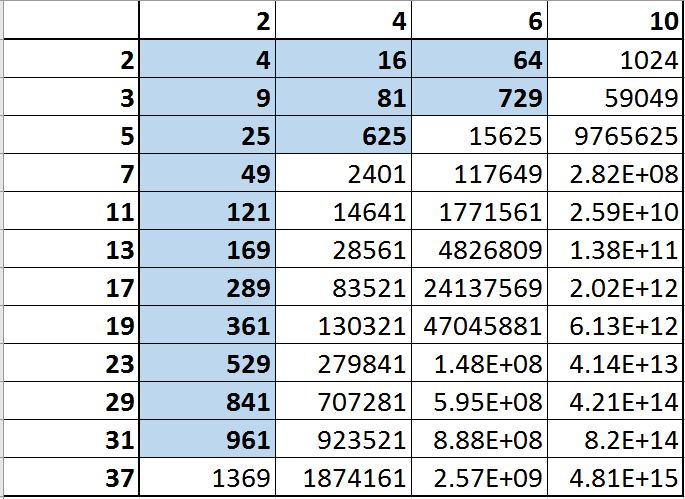
\includegraphics{prime}
\end{center}

From this table, we can see that our answer is that there are \(\boxed{16}\) non-prime numbers below \(1000\) with a prime number of factors.
\newpage

\section{Borel's Other Paradox}
\subsection{Problem}
You have a ruler, with \(0\) and \(1\) marked at either end. You also have a roll of tape, the same width as the ruler.

First you cut a piece of tape of length \(\frac{1}{8}\), and stick it with its centre at position \(\frac{1}{2}\). This tape covers the ruler from \(\frac{7}{16}\) to \(\frac{9}{16}\).

You then stick pieces of tape of length \(\frac{1}{27}\), centred at positions \(\frac{1}{3}\) and \(\frac{2}{3}\).

You carry on in this way, sticking pieces of tape of length \(\frac{1}{q^3}\) at every fraction \(\frac{p}{q}\) lying between \(0\) and \(1\), regardless of whether there is any tape there already.

By the end of this (infinite) process, are all points of the ruler covered?

\subsection{Hint}
You may wish to use the fact that \[\frac{1}{1^2}+\frac{1}{2^2}+\frac{1}{3^2}+...=\frac{\pi^2}{6}\]
\subsection{Solution}
Let us consider the total length of tape used.

As an example, let us consider the fifths. We use \(\frac{1}{5^3}\), for each of the fifths between \(0\) and \(1\): \(\frac{1}{5}\), \(\frac{2}{5}\), \(\frac{3}{5}\) and \(\frac{4}{5}\). The total length of this tape, \(L_5\) is:

\[L_5=\frac{5-1}{5^3}\]

In general, for nths, the length of tape used is \(L_n\)

\[L_n=\frac{n-1}{n^3}\]

So the total length of tape used, \(L_{total}\), is

\[L_{total}=\frac{1}{2^3}+\frac{2}{3^3}+\frac{3}{4^3}+...\]

Each of these terms \(\frac{n-1}{n^3}\) is less than \(\frac{n}{n^3}=\frac{1}{n^2}\), so,

\[L_{total}=\frac{1}{2^3}+\frac{2}{3^3}+\frac{3}{4^3}+...\leq \frac{1}{2^2}+\frac{1}{3^2}+\frac{1}{4^2}+...\]

but,

\[\frac{1}{1^2}+\frac{1}{2^2}+\frac{1}{3^2}+...=\frac{\pi^2}{6}\]

so,

\[\frac{1}{2^2}+\frac{1}{3^2}+\frac{1}{4^2}+...=\frac{\pi^2}{6}-1\]

We have therefore found that:

\[L_{total} \leq \frac{\pi^2}{6}-1\]

So, the total length of tape used was less than \(1\), which means the entire ruler cannot be covered.
\subsection{Extension}
How much tape was used?

How much of the ruler was covered? (I think this might be very hard)


\newpage

\section{Tetrahedrons and Pyramids}
\subsection{Problem}
\subsection{Solution}
\newpage

\section{Robo Vision}
\subsection{Problem}
\subsection{Solution}
\newpage


\section{The Problem with Socks}
\subsection{Problem}
\subsection{Solution}

\newpage
\section{Check Digits}
\subsection{Problem}
\subsection{Solution}
\newpage
\section{Cube inside sphere inside cube}
\subsection{Problem}
\subsection{Solution}

\newpage
\section{Is \(n^3-n\) divisible by 6?}
\subsection{Problem}
\subsection{Solution}


\newpage
\section{The Surgeon's Gloves}
\subsection{Problem}
\subsection{Solution}
\end{document}
